This dissertation investigates the intersection of Black sonic epistemologies, digital tools, and embodied interaction through the methodological framework of \textit{Sonic Speculocultural Technopoiesis}. It follows the traditional structure of dissertation research (introduction, literature review, methodology, results, discussion, conclusion), while being internally organized through the cyclical domains of \textbf{Unsettling}, \textbf{Remixing}, \textbf{Embodying}, and \textbf{Transmitting}.

%%%%%%%%%%%%%%%%%%%% TABLE FOR CHAPTER DESCRIPTIONS %%%%%%%%%%%%%%%%%%%%%%%%%%%%%
\begin{figure}[H] 
	\hspace*{-0.5in}  % Adjust the value as needed
	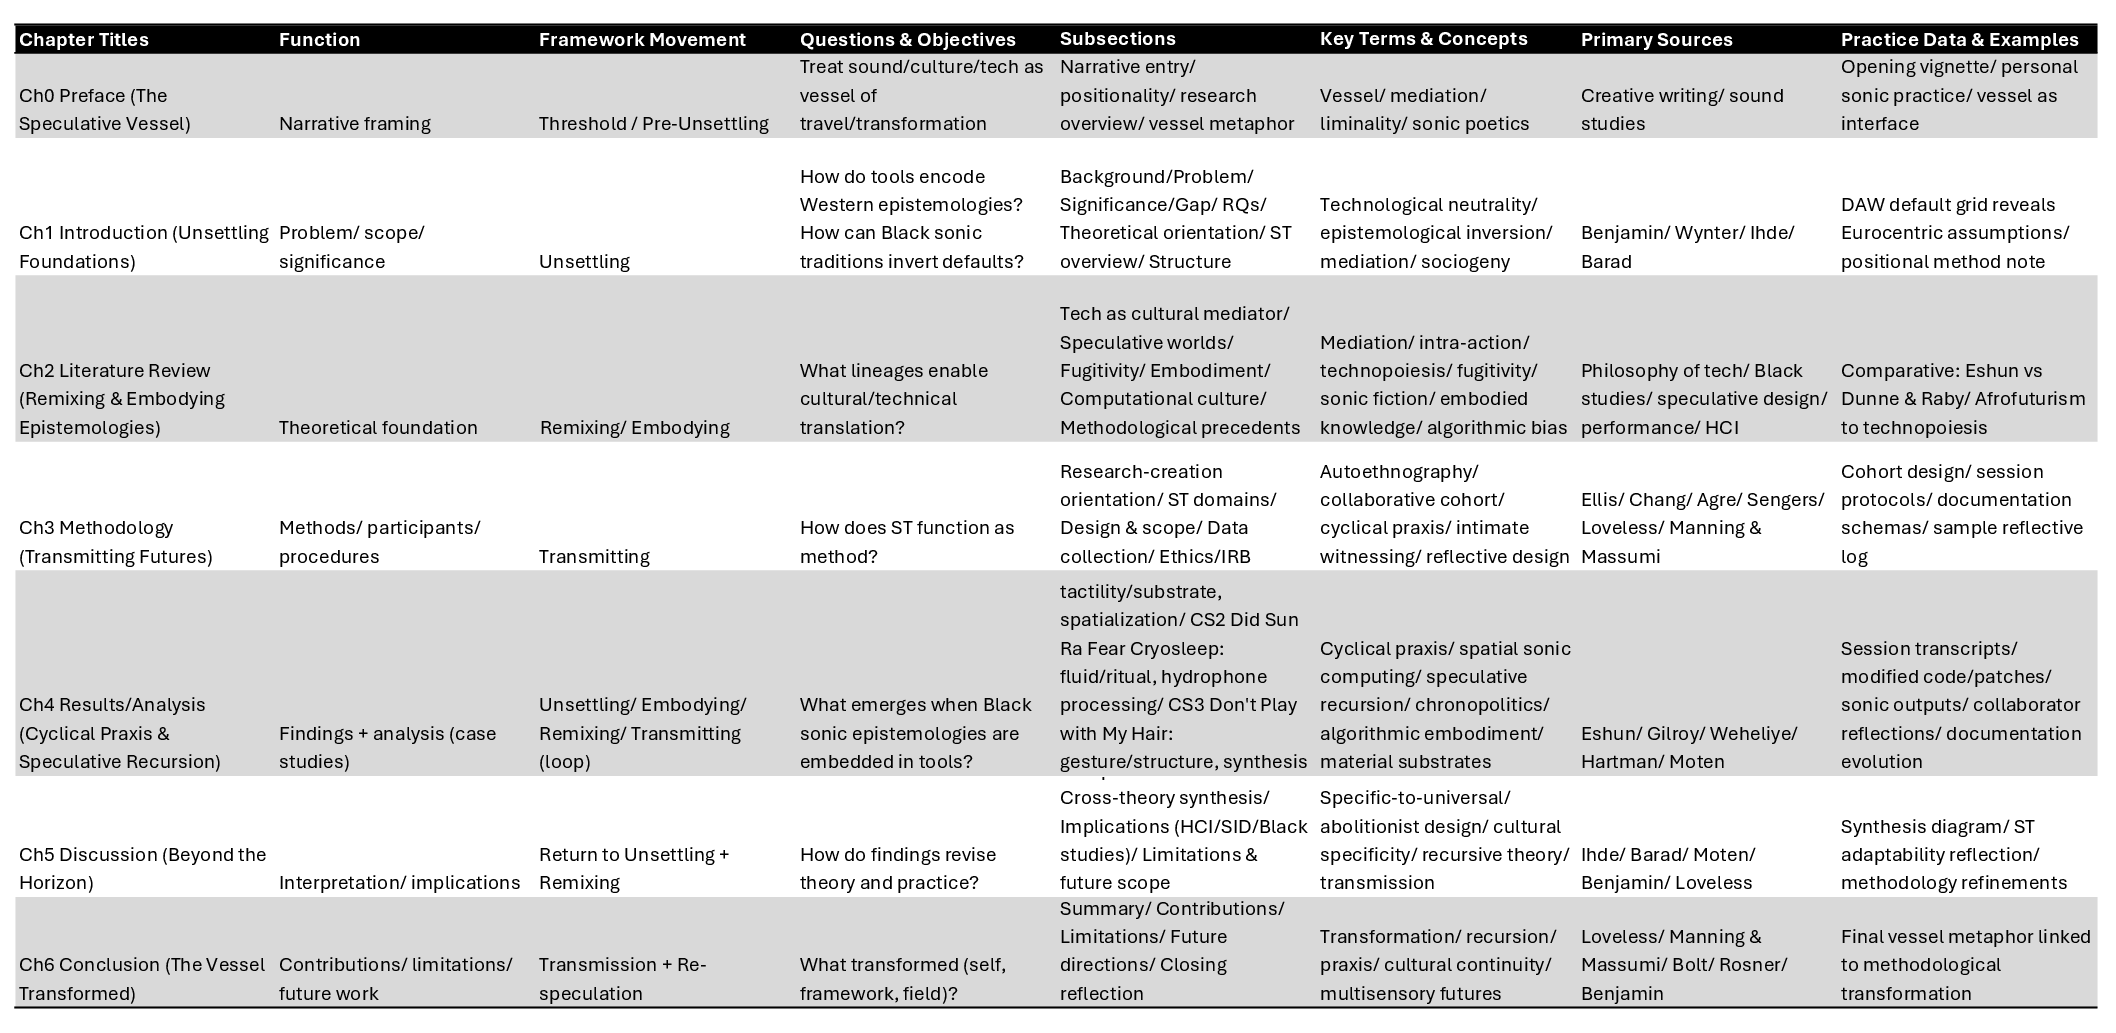
\includegraphics[width=1.15\textwidth]{assets/tables/table_5_1_chapterMatrix.png} 
	\captionof{table}{Dissertation Chapter Matrix} 
	\label{tab:chapter-matrix} 
\end{figure}

\begin{comment}
\begin{itemize}
\item \textbf{Preface:} The Speculative Vessel — A short narrative entry-point, framing the dissertation as a journey through speculative vessels of sound, culture, and technology.
\item \textbf{Chapter 1:} Introduction (Unsettling) — Establishes the research problem, significance, and scope. Confronts Western paradigms of technological neutrality and introduces epistemological inversion through Black studies critiques (Benjamin, Wynter, Ihde).
\item \textbf{Chapter 2:} Literature Review (Remixing and Embodying) — Provides the theoretical grounding across multiple traditions: post-phenomenology, agential realism, speculative design, Afrofuturism, fugitivity, embodiment, sonic practices, and computational culture. Draws on Black radical thought (Moten, Hartman, Robinson, Gilroy, Weheliye) to establish remix and embodiment as methodological logics.
\item \textbf{Chapter 3:} Methodology (Transmitting) — Explains the methodological framework: autoethnography, collaborative design, reflective design, critical technical practice (CTP), and research-creation. Demonstrates how collaborative sonic sessions function as sites of transmission and cultural preservation.
\item \textbf{Chapter 4:} Results and Analysis (Cyclical Praxis and Speculative Recursion) —  Presents findings from workshops and major case studies. Demonstrating the full cycle of ST in practice through spatial sonic computing. The works come to fruition via enacting speculative recursion, refining the framework through experimentation.
\begin{itemize}
	\item \emph{Buffalo Soldier}
	\item \emph{Did Sun Ra Fear Cryosleep?}
\end{itemize}
\item \textbf{Chapter 5:} Discussion — Interprets the case study findings through the theoretical lenses established earlier. Reflects on adaptability, specificity, and limitations of the framework. Positions ST as a model grounded in Black sonic epistemologies, yet with potential adaptability to other epistemic traditions.
\item \textbf{Chapter 6:} Conclusion (The Vessel Transformed) — Returns to the metaphor of the vessel. Summarizes contributions, acknowledges limitations, and offers directions for future research and practice. Shows the metamorphosis and transfiguration of the vessel, self, and knowledge through the dissertation journey.
\end{itemize}
\end{comment}


